\def\languageisenglish{}

\subimport{../Layout/}{FAQ_layout.tex}

\newcommand{\booktitle}{FAQ and Errata}
\newcommand{\forversion}{For v1.3.5}
\newcommand{\faqversion}{Version 1}
\hypersetup{pdftitle={T9A - \booktitle}}

% Care to use the latest .tex files for up-to-date references - they need to be compiled
\externaldocument{../Rules/FB_T9A_Rules_1-3-5_EN}
\externaldocument{../Paths/FB_T9A_Paths_1-3-5_EN}

\begin{document}

\newcommand{\howtousethisdocumenttitle}{How to use this document}
\newcommand{\howtousethisdocumenttext}{%
While we always strive to provide books of the highest quality, inadvertent mistakes and unforeseen consequences in rules interaction tend to find their way into the documents. This FAQ document was created to answer some of the most common or complicated questions.
}
\newcommand{\recentchangessentence}{%
Recent changes are colour-coded like this sentence.
}

\subimport{../Layout/}{FAQ_titlepage.tex}

\clearpage

\basicbigtitle{Errata}

\basictitle{Rulebook}

\erratatitle{Walls}{\getpage{walls}}
\erratatext{%
Add to \textbf{Defending a Wall}:\newline
\enquote{If a unit has more than half of its models in a facing that is in base contact with a Wall, all \rnf{} models in this unit count as defending this Wall.}
}

\newerratatitle{Counterthrust}{\getpage{counterthrust}}
\newerratatext{%
\textbf{Change:} \enquote{\textit{No unit can be deployed within \distance{18} of an enemy unit (excluding special deployment such as Scouts).}}\newline
\textbf{To:} \enquote{Units must be deployed more than \distance{18} of an enemy unit (excluding special deployment such as Scouts).}
}

\basictitle{Armybooks}

\basicsubtitle{Beast Herds}

\erratatitle{Hunting Call}{5}
\erratatext{%
\textbf{Change:} \enquote{\textit{Ambush rolls for such units must be made at the beginning of Game Turn 1.}}\newline
\textbf{To:} \enquote{Ambush rolls for such units must be made at the beginning of the Remaining Moves sub-phase of the controlling player's Player Turn 1.}
}

\basicbigtitle{F.A.Q.}

\basictitle{Rulebook}

\questiontitle{Charge Reactions}{\getpage{chargereaction}}
\QandA{%
Must a unit immediately resolve their Charge Reaction at the same time as they declare it?
}{%
Yes.
}

\questiontitle{Miscast}{\getpage{table/miscast}}
\QandA{%
In what order are Miscast effects applied?
}{%
Apply the effects of the Miscast Table from top to bottom. So the order is Witch Fire > Amnesia > Catastrophic
Detonation > Breach in the Veil.
}

\questiontitle{Recover Wounds and Raise Wounds}{\getpage{recoverandraisewounds}}
\QandA{%
Can single model units place Raised models beside the one model in a rank, or do they have to be placed behind it?
}{%
They can be placed in the first rank. Single model units are one rank units, so the first rank is the back rank for Raising purposes.
}

\additionalQandA{%
How do Raised models interact with ongoing effects on their unit (Fleeing, Spells, Charge Bonuses, etc.)?
}{%
Raised models are subject to the same ongoing effects as their unit, and count as Charging if their unit Charged.
}

\questiontitle{Pursuits and Overruns}{\getpage{pursuits_and_overruns}}
\QandA{%
In a Combat involving multiple units from each side, do all units on the winning side have to Pursue the same Fleeing enemy unit?
}{%
No. Each Pursuing unit may choose any eligible enemy unit to Pursue.
}

\questiontitle{Combat Reforms}{\getpage{combatreform}}
\QandA{%
Can you bring friendly units into base contact with each other during a Combat Reform?
}{%
Yes. The restriction regarding not moving into base contact with new units only applies to new enemy units.
}

\additionalQandA{%
When Combat Reforming with multiple units, when do I check that the exact same enemy models are still in base contact with an enemy?
}{%
Check once all Combat Reforms for all your units have been completed. Remember that after each Reform the reforming units must have the same number of models in base contact, and no Character can move out of base contact.
}

\questiontitle{Accepting or Refusing a Challenge}{\getpage{accepting_or_refusing_a_challenge}}
\QandA{%
Can a model accept a Challenge if it is not in base contact with the unit of a model issuing a Challenge? Can they be nominated as the model chosen as refusing the Challenge if the Challenge is refused?
}{%
Yes, so long as the model accepting or being nominated is in a unit in base contact with the Challenge issuer's unit. When accepting and being nominated as the Character that refused a Challenge, the requirement is that the model's unit must be in base contact with the unit of the model issuing the Challenge, not that the model itself be in base contact with the unit of the model issuing the Challenge. The text in parentheses in the paragraph \nameref*{issuing_a_challenge} on page \pageref*{issuing_a_challenge} should state \enquote{this model, or its unit, must be in base contact with}. Note that being in brackets, this was not a rule but a reminder and has no authority to alter what is written in the rules defining a Challenge.
}

\questiontitle{Special Attacks}{\getpage{special_attacks}}
\QandA{%
Can Special Attacks be modified by other special rules that do not specifically \enquote{benefit} the Special Attack?
}{%
No. Special rules do not affect Special Attacks, regardless of whether they benefit the attack or not. For instance, a Chariot's Impact Hits would not be reduced in Strength by the Chill Aura of a Frost Phoenix.
}

\questiontitle{Jack's Pickaxe}{\getpage{magical_weapons}}
\QandA{%
Does Jack's Pickaxe gain its +1 Strength bonus against models with Towering Presence?
}{%
Yes. Against models with Towering Presence, Jack's Pickaxe rolls to wound with a strength equal to target's T+1. For example, a Strength 4 model attacking a Toughness 6 model with Towering Presence would count as having Strength 7 when rolling to wound. Note that for modifying Armour Saves, a model with Jack's Pickaxe still only counts as having their normal Strength plus 1.
}

\questiontitle{Wizard's Hood}{\getpage{enchanted_items}}
\QandA{%
What happens if the Enchanted Item Wizard's Hood is destroyed or temporarily ceases to work?
}{%
The bearer of the item is no longer a Wizard (which means the bearer cannot Cast or Dispel Spells, or Channel). If the bearer carries a Magical Item that only Wizards can use (such as a Dispel Scroll, since only Wizards can dispel), it can no longer use this item. If it is a temporary effect, such as when interacting with Mikinok's Totem from the Orcs and Goblins Armybook, the bearer becomes a Wizard Apprentice again and regains the ability to use Wizard-only Magical Items as soon as the effect stops. The bearer does not roll again for Spells or Path.
}

\questiontitle{Failed Charge}{\getpage{failed_charge}}
\QandA{%
Can Failed Charge Moves ignore the Unit Spacing rule?
}{%
No. Failed Charge Moves are not Charge Moves and thus do not ignore the Unit Spacing rule. Sometimes this means units cannot move their full Failed Charge distance. For example, if other units or terrain are too close to allow the Failed Charging unit to Wheel enough to have their target's centre directly in front of it, the unit Wheels as much as it can and then moves no further. Remember that the Unit Spacing rule allows units to be temporarily within \distance{½} as long as they end their move more than \distance{1} away.
}

\questiontitle{Priority of Modifiers}{\getpage{priority_of_modifiers}}
\QandA{%
When two or more effects that should always dictate the result of a dice roll contradict each other, such as a model with The Bigger They Are (always wound on a 4+ or better) attacking a model under the effect of \shamanismattribute{} (cannot be wounded on better than a 5+), which effect should be applied?
}{%
Apply the effect resulting in the lowest chance of success (in the example, \shamanismattribute{}).
}

\questiontitle{Essence of a Free Mind}{\getpage{arcane_items}}
\QandA{%
When does a Character with Essence of a Free Mind decide which Path to generate spells from?
}{%
Immediately before they generate their spells.
}

\questiontitle{Ruins}{\getpage{ruins}}
\QandA{%
If a Cavalry, Monstrous Cavalry or Chariot unit with Skirmishers triggers a Dangerous Terrain (2) Test in Ruins, do
they ignore it as other Skirmishers ignore Dangerous Terrain (1)?
}{%
Yes.
}

\questiontitle{Blocked Path}{\getpage{blocked_path}}
\QandA{%
When using the Blocked Path rules and performing the enemy unit Reform, can the move be performed so that the Charging unit ends up being Engaged in a Facing other than its front?
}{%
No. The Charging unit must be Engaged in its front.
}

\questiontitle{Supporting Attacks}{\getpage{supporting_attacks}}
\QandA{%
In a unit with an incomplete rear rank, can these models move over to maximise Supporting Attacks?
}{%
No. The models remain where they are placed unless they are forced to change position due to a Reform, a Character leaving or joining the unit, models with the Front Rank rule shifting during an Advance or March Move, a Make Way move, or as the result of casualties to a \rnf{} unit with different \rnf{} Troop Types (such as Skinks and Caimans).
}

\questiontitle{Swirling Melee}{\getpage{swirling_melee}}
\QandA{%
If a \rnf{} model is only in contact with a Character in a Challenge, and that Character is part of a combined unit, can the \rnf{} model still use Swirling Melee to allocate attacks towards enemy \rnf{}?
}{%
Yes.
}

\questiontitle{Penetrating}{\getpage{penetrating}}
\QandA{%
If a model with Penetrating is between two arcs of its target unit, which arc does it count as being in for the purpose
of determining hits?
}{%
The arc which it has the centre of its base in (in case of a tie, randomise which arc it is in).
}

\questiontitle{Leaving a combined unit \&{} Charging out of a unit}{\getpage{leaving_a_combined_unit}}
\QandA{%
What effects count as \enquote{movement alterations} when a Character leaves a unit?
}{%
Only modifiers to the Movement Characteristic. All other effects connected to moving, but not modifiers to the Characteristics value (such as Strider, Fly, Ethereal, etc.), are lost as soon as the Character physically leaves the unit.
Note that rules affecting Charge Range rolls (such as Swiftstride) can still be used when charging out of a unit, as these are rolled while the Character is still in the unit.
}

\questiontitle{Bound Spells}{\getpage{bound_spells}}
\QandA{%
Will casting a Bound Spell trigger its Path's Attribute Spell?
}{%
Yes.
}

\begin{minipage}[c]{0.65\textwidth}\newquestiontitle{Unit Facing and Arcs}{\getpage{unit_facing_and_arcs}}
\vspace*{1ex}
\newQandA{%
If model A has a single point of its base on the line that separates two arcs of model B, which arc is A in?
}{%
It is considered to be (partly) in both arcs.\newline
See example to the right. The orange model has a corner of its base tangent to the purple model's Front Arc. The orange model is considered to be in the Front Arc of the purple unit.
}\end{minipage}\hfill\begin{minipage}[c]{0.27\textwidth}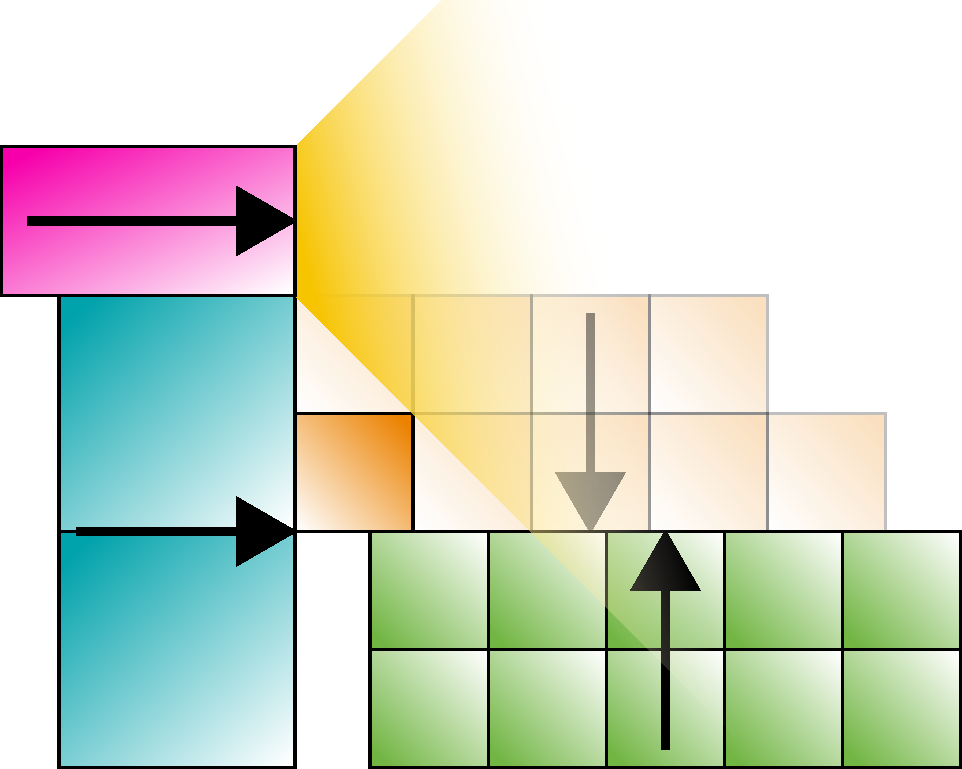
\includegraphics[width=\textwidth]{tangent_line_of_sight.pdf}\end{minipage}

\basictitle{Paths of Magic}

\basicsubtitle{Witchcraft}

\questiontitle{\witchcraftspelltwo}{\getpage{witchcraft}}
\QandA{%
Can a model use a Shooting Attack with the Move or Fire rule after moving with \witchcraftspelltwo{}?
}{%
No. While the Reform from this spell does not prevent a model from Shooting, normal restrictions on Shooting apply to the Magical Move itself.
}

\questiontitle{\witchcraftspellthree}{\getpage{witchcraft}}
\QandA{%
Is the minimum range for Shooting Attacks and Spells also halved?
}{%
Yes.
}

\basicsubtitle{\newrule{Druidism}}

\newquestiontitle{\druidismspellone}{\getpage{druidism}}
\newQandA{%
Do Buildings count as Impassable Terrain for the purposes of measuring the Range of \druidismspellone{}?
}{%
Yes.
}

\basicsubtitle{\newrule{Evocation}}

\newquestiontitle{\evocationspelltwo}{\getpage{evocation}}
\newQandA{%
If you move into contact with a model with Ricochet using \evocationspelltwo{}, do you get a \wardsave{3+} against the wounds caused?
}{%
Yes.
}

\basictitle{Armybooks}

\basicsubtitle{Dread Elves}

\questiontitle{Divine Altar}{16}
\QandA{%
How many different effects can a Divine Altar choose from for its Divine Blessing rule?
}{%
Three different effects: Lethal Strike, Ward Save against Artillery Weapons or rerolling Charge Range.
}

\newpage
\basicsubtitle{\newrule{Dwarven Holds}}

\newquestiontitle{Ancient Grudge}{2}
\newQandA{%
When a unit containing a Character at Deployment is Begrudged, is the Character still begrudged if it leaves the unit?
}{%
Yes. All models (including Characters, War Platforms, etc.) in a unit at the time it is begrudged are treated as the
target of the Ancient Grudge.
}

\basicsubtitle{Infernal Dwarves}

\questiontitle{Wall of Lead}{3}
\QandA{%
Is Wall of Lead a rule for the Blunderbuss?
}{%
Yes.
}

\questiontitle{Bound Daemon}{14}
\QandA{%
Does a Titan Mortar's Ogre Slave count as a crew when taking the Bound Daemon upgrade?
}{%
Yes. Thus it is lost.
}

\basicsubtitle{Highborn Elves}

\questiontitle{Fire Phoenix}{19}
\QandA{%
If a Fire Phoenix passes its Rebirth roll on the last turn of the game, does it count as a casualty for Victory Points?
}{%
Yes. Since the Fire Phoenix could not be placed on the table, it counts as a casualty.
}

\basicsubtitle{Ogre Khans}

\questiontitle{Mammoth-Hide Cloak}{4}
\QandA{%
When does the modifier from the Mammoth-Hide Cloak take effect?
}{%
The Strength of any \textbf{hits} is modified, so the Cloak reduces the Strength to 5 after all other modifications to the Strength of an attack have been made.
}

\basicsubtitle{\newrule{Saurian Ancients}}

\newquestiontitle{Ancient Knowledge \&{} Wandering Path}{5}
\newQandA{%
Can a model with Ancient Knowledge and Wandering Path take spells from a Path other than Divination?
}{%
No.
}

\basicsubtitle{\newrule{Sylvan Elves}}

\newquestiontitle{Tree Singing}{2}
\newQandA{%
Does a forest (and eligible friendly units) targeted by Tree Singing have to move the full \distance{D3+3} or can you opt to move less than the rolled distance?
}{%
Both the forest and all eligible friendly units have to move the full distance unless the move would bring the
target(s) into contact with enemy units or other Terrain Features. In this case it immediately stops before moving into contact. Note that the targets of the spell do not change formation or the direction in which they are facing, as no manoeuvres (e.g. Pivots, Wheels, Reforms), other than this move may be performed.
}

\newpage
\basicsubtitle{\newrule{Undying Dynasties}}

\newquestiontitle{Commander of the Terracotta Army}{5}
\newQandA{%
Can a Pharaoh that loses Flammable (due to being from a Terracotta army) gain Flammable again from other sources (for example via the Alchemy Attribute).
}{%
Yes.
}

\newquestiontitle{Mummy's Curse}{6}
\newQandA{%
If a Pharaoh or Nomarch is removed as a casualty as a result of Unstable, how is Mummy's Curse carried out?
}{%
No model caused the final wound. The Mummy's Curse has no effect.
}

\end{document}
